% Options for packages loaded elsewhere
\PassOptionsToPackage{unicode}{hyperref}
\PassOptionsToPackage{hyphens}{url}
%
\documentclass[
]{article}
\usepackage{amsmath,amssymb}
\usepackage{lmodern}
\usepackage{iftex}
\ifPDFTeX
  \usepackage[T1]{fontenc}
  \usepackage[utf8]{inputenc}
  \usepackage{textcomp} % provide euro and other symbols
\else % if luatex or xetex
  \usepackage{unicode-math}
  \defaultfontfeatures{Scale=MatchLowercase}
  \defaultfontfeatures[\rmfamily]{Ligatures=TeX,Scale=1}
\fi
% Use upquote if available, for straight quotes in verbatim environments
\IfFileExists{upquote.sty}{\usepackage{upquote}}{}
\IfFileExists{microtype.sty}{% use microtype if available
  \usepackage[]{microtype}
  \UseMicrotypeSet[protrusion]{basicmath} % disable protrusion for tt fonts
}{}
\makeatletter
\@ifundefined{KOMAClassName}{% if non-KOMA class
  \IfFileExists{parskip.sty}{%
    \usepackage{parskip}
  }{% else
    \setlength{\parindent}{0pt}
    \setlength{\parskip}{6pt plus 2pt minus 1pt}}
}{% if KOMA class
  \KOMAoptions{parskip=half}}
\makeatother
\usepackage{xcolor}
\usepackage[margin=1in]{geometry}
\usepackage{color}
\usepackage{fancyvrb}
\newcommand{\VerbBar}{|}
\newcommand{\VERB}{\Verb[commandchars=\\\{\}]}
\DefineVerbatimEnvironment{Highlighting}{Verbatim}{commandchars=\\\{\}}
% Add ',fontsize=\small' for more characters per line
\usepackage{framed}
\definecolor{shadecolor}{RGB}{248,248,248}
\newenvironment{Shaded}{\begin{snugshade}}{\end{snugshade}}
\newcommand{\AlertTok}[1]{\textcolor[rgb]{0.94,0.16,0.16}{#1}}
\newcommand{\AnnotationTok}[1]{\textcolor[rgb]{0.56,0.35,0.01}{\textbf{\textit{#1}}}}
\newcommand{\AttributeTok}[1]{\textcolor[rgb]{0.77,0.63,0.00}{#1}}
\newcommand{\BaseNTok}[1]{\textcolor[rgb]{0.00,0.00,0.81}{#1}}
\newcommand{\BuiltInTok}[1]{#1}
\newcommand{\CharTok}[1]{\textcolor[rgb]{0.31,0.60,0.02}{#1}}
\newcommand{\CommentTok}[1]{\textcolor[rgb]{0.56,0.35,0.01}{\textit{#1}}}
\newcommand{\CommentVarTok}[1]{\textcolor[rgb]{0.56,0.35,0.01}{\textbf{\textit{#1}}}}
\newcommand{\ConstantTok}[1]{\textcolor[rgb]{0.00,0.00,0.00}{#1}}
\newcommand{\ControlFlowTok}[1]{\textcolor[rgb]{0.13,0.29,0.53}{\textbf{#1}}}
\newcommand{\DataTypeTok}[1]{\textcolor[rgb]{0.13,0.29,0.53}{#1}}
\newcommand{\DecValTok}[1]{\textcolor[rgb]{0.00,0.00,0.81}{#1}}
\newcommand{\DocumentationTok}[1]{\textcolor[rgb]{0.56,0.35,0.01}{\textbf{\textit{#1}}}}
\newcommand{\ErrorTok}[1]{\textcolor[rgb]{0.64,0.00,0.00}{\textbf{#1}}}
\newcommand{\ExtensionTok}[1]{#1}
\newcommand{\FloatTok}[1]{\textcolor[rgb]{0.00,0.00,0.81}{#1}}
\newcommand{\FunctionTok}[1]{\textcolor[rgb]{0.00,0.00,0.00}{#1}}
\newcommand{\ImportTok}[1]{#1}
\newcommand{\InformationTok}[1]{\textcolor[rgb]{0.56,0.35,0.01}{\textbf{\textit{#1}}}}
\newcommand{\KeywordTok}[1]{\textcolor[rgb]{0.13,0.29,0.53}{\textbf{#1}}}
\newcommand{\NormalTok}[1]{#1}
\newcommand{\OperatorTok}[1]{\textcolor[rgb]{0.81,0.36,0.00}{\textbf{#1}}}
\newcommand{\OtherTok}[1]{\textcolor[rgb]{0.56,0.35,0.01}{#1}}
\newcommand{\PreprocessorTok}[1]{\textcolor[rgb]{0.56,0.35,0.01}{\textit{#1}}}
\newcommand{\RegionMarkerTok}[1]{#1}
\newcommand{\SpecialCharTok}[1]{\textcolor[rgb]{0.00,0.00,0.00}{#1}}
\newcommand{\SpecialStringTok}[1]{\textcolor[rgb]{0.31,0.60,0.02}{#1}}
\newcommand{\StringTok}[1]{\textcolor[rgb]{0.31,0.60,0.02}{#1}}
\newcommand{\VariableTok}[1]{\textcolor[rgb]{0.00,0.00,0.00}{#1}}
\newcommand{\VerbatimStringTok}[1]{\textcolor[rgb]{0.31,0.60,0.02}{#1}}
\newcommand{\WarningTok}[1]{\textcolor[rgb]{0.56,0.35,0.01}{\textbf{\textit{#1}}}}
\usepackage{graphicx}
\makeatletter
\def\maxwidth{\ifdim\Gin@nat@width>\linewidth\linewidth\else\Gin@nat@width\fi}
\def\maxheight{\ifdim\Gin@nat@height>\textheight\textheight\else\Gin@nat@height\fi}
\makeatother
% Scale images if necessary, so that they will not overflow the page
% margins by default, and it is still possible to overwrite the defaults
% using explicit options in \includegraphics[width, height, ...]{}
\setkeys{Gin}{width=\maxwidth,height=\maxheight,keepaspectratio}
% Set default figure placement to htbp
\makeatletter
\def\fps@figure{htbp}
\makeatother
\setlength{\emergencystretch}{3em} % prevent overfull lines
\providecommand{\tightlist}{%
  \setlength{\itemsep}{0pt}\setlength{\parskip}{0pt}}
\setcounter{secnumdepth}{-\maxdimen} % remove section numbering
\usepackage{booktabs}
\usepackage{longtable}
\usepackage{array}
\usepackage{multirow}
\usepackage{wrapfig}
\usepackage{float}
\usepackage{colortbl}
\usepackage{pdflscape}
\usepackage{tabu}
\usepackage{threeparttable}
\usepackage{threeparttablex}
\usepackage[normalem]{ulem}
\usepackage{makecell}
\usepackage{xcolor}
\ifLuaTeX
  \usepackage{selnolig}  % disable illegal ligatures
\fi
\IfFileExists{bookmark.sty}{\usepackage{bookmark}}{\usepackage{hyperref}}
\IfFileExists{xurl.sty}{\usepackage{xurl}}{} % add URL line breaks if available
\urlstyle{same} % disable monospaced font for URLs
\hypersetup{
  pdftitle={Data Cleaning and Preprocessing},
  hidelinks,
  pdfcreator={LaTeX via pandoc}}

\title{Data Cleaning and Preprocessing}
\author{}
\date{\vspace{-2.5em}2023-03-06}

\begin{document}
\maketitle

\hypertarget{read-data-and-load-packages}{%
\section{Read Data and Load
Packages}\label{read-data-and-load-packages}}

\begin{Shaded}
\begin{Highlighting}[]
\CommentTok{\# load important packages}
\NormalTok{pacman}\SpecialCharTok{::}\FunctionTok{p\_load}\NormalTok{(}
\NormalTok{  tidyverse, naniar, dlookr, DataExplorer, janitor, tidymodels}
\NormalTok{  )}


\CommentTok{\#read in the csv file and clean the column names}
\NormalTok{vgsales\_df }\OtherTok{\textless{}{-}} \FunctionTok{read\_csv}\NormalTok{(}
  \StringTok{"datasets/vgsales{-}12{-}4{-}2019.csv"}\NormalTok{, }\AttributeTok{show\_col\_types =}\NormalTok{ F}
\NormalTok{  ) }\SpecialCharTok{\%\textgreater{}\%}   
  \CommentTok{\# start with cleaning column names into a consistent convention}
  \FunctionTok{clean\_names}\NormalTok{()}
\end{Highlighting}
\end{Shaded}

\begin{Shaded}
\begin{Highlighting}[]
\CommentTok{\#this code is used to show the percentage of missing values in each variable}
\FunctionTok{gg\_miss\_var}\NormalTok{(vgsales\_df,}\AttributeTok{show\_pct =}\NormalTok{ T)}\SpecialCharTok{+}
  \FunctionTok{labs}\NormalTok{(}\AttributeTok{title =} \StringTok{"\% missingness by variable"}\NormalTok{)}
\end{Highlighting}
\end{Shaded}

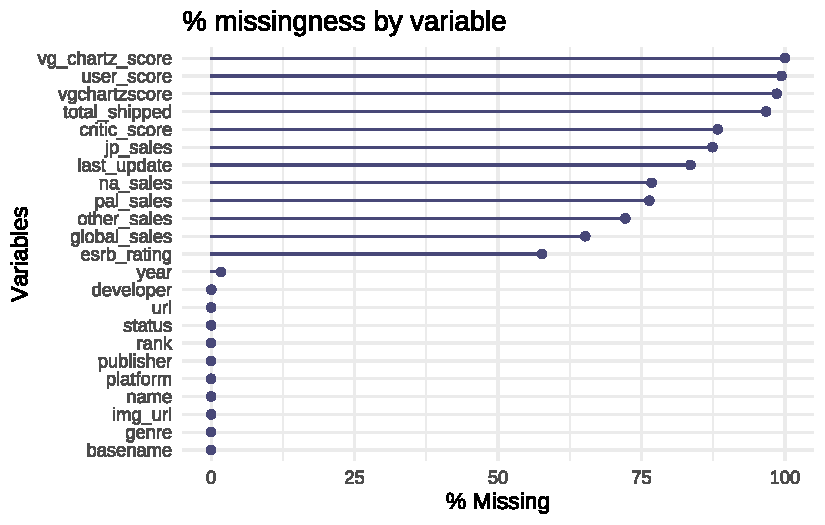
\includegraphics{cleaning-pipeline_files/figure-latex/unnamed-chunk-2-1.pdf}

\begin{Shaded}
\begin{Highlighting}[]
\CommentTok{\# create a report using the data in vgsales\_df, }
\CommentTok{\# output the report in html format, name the report vgsales\_eda.html, }
\CommentTok{\# and save the report in the current working directory}
\FunctionTok{create\_report}\NormalTok{(}
  \AttributeTok{data =}\NormalTok{ vgsales\_df, }
  \AttributeTok{output\_format =} \StringTok{"html\_document"}\NormalTok{, }
  \AttributeTok{output\_file =} \StringTok{"vgsales\_eda.html"}\NormalTok{, }
  \AttributeTok{output\_dir =} \StringTok{"./"}
\NormalTok{)}
\end{Highlighting}
\end{Shaded}

\begin{Shaded}
\begin{Highlighting}[]
\CommentTok{\# find out the count of genre by year(which year which genre sold more)}
\NormalTok{vgsales\_df }\SpecialCharTok{\%\textgreater{}\%} 
  \FunctionTok{count}\NormalTok{(year, genre, }\AttributeTok{sort =}\NormalTok{ T) }\SpecialCharTok{\%\textgreater{}\%} 
  \CommentTok{\# filter first 10 results}
  \FunctionTok{slice\_head}\NormalTok{(}\AttributeTok{n =} \DecValTok{10}\NormalTok{)}
\end{Highlighting}
\end{Shaded}

\begin{verbatim}
## # A tibble: 10 x 3
##     year genre         n
##    <dbl> <chr>     <int>
##  1  2014 Misc       1273
##  2  2013 Misc        936
##  3  2009 Misc        844
##  4  2012 Misc        721
##  5  2010 Misc        673
##  6  2011 Misc        671
##  7  2009 Action      572
##  8  2008 Misc        496
##  9  2009 Adventure   481
## 10  2011 Action      480
\end{verbatim}

\begin{Shaded}
\begin{Highlighting}[]
\CommentTok{\# prepare data for modeling with sales as the target variable}


\NormalTok{vgsales\_df\_clean }\OtherTok{\textless{}{-}}\NormalTok{ vgsales\_df }\SpecialCharTok{\%\textgreater{}\%}
  \CommentTok{\# remove columns that are not needed for analysis }
  \CommentTok{\# please refer to the above eda report on the missing variable part}
  \FunctionTok{select}\NormalTok{(}
    \SpecialCharTok{{-}}\FunctionTok{c}\NormalTok{(basename, url, img\_url, vg\_chartz\_score, vgchartzscore, }
\NormalTok{       user\_score, total\_shipped, critic\_score, last\_update)}
\NormalTok{    ) }\SpecialCharTok{\%\textgreater{}\%} 
   \CommentTok{\# change character columns to factors}
  \FunctionTok{mutate\_if}\NormalTok{(is.character, as.factor) }\SpecialCharTok{\%\textgreater{}\%} 
  \CommentTok{\# reduce factor levels of genre, esrb\_rating, platform, developer}
  \CommentTok{\# also refer to the charts in the eda report }
  \CommentTok{\#to see the most common levels in each factor variable}
  \FunctionTok{mutate}\NormalTok{(}
    \AttributeTok{genre =} \FunctionTok{fct\_lump\_n}\NormalTok{(genre, }\AttributeTok{n =} \DecValTok{10}\NormalTok{, }\AttributeTok{other\_level =} \StringTok{"Other"}\NormalTok{),}
    \AttributeTok{esrb\_rating =} \FunctionTok{fct\_lump\_n}\NormalTok{(esrb\_rating, }\AttributeTok{n =} \DecValTok{4}\NormalTok{, }\AttributeTok{other\_level =} \StringTok{"Other"}\NormalTok{),}
    \AttributeTok{platform =} \FunctionTok{fct\_lump\_n}\NormalTok{(platform, }\AttributeTok{n =} \DecValTok{10}\NormalTok{, }\AttributeTok{other\_level =} \StringTok{"Other"}\NormalTok{),}
    \AttributeTok{developer =} \FunctionTok{fct\_lump\_n}\NormalTok{(developer, }\AttributeTok{n =} \DecValTok{10}\NormalTok{, }\AttributeTok{other\_level =} \StringTok{"Other"}\NormalTok{),}
    \AttributeTok{publisher =} \FunctionTok{fct\_lump\_n}\NormalTok{(publisher, }\AttributeTok{n =} \DecValTok{10}\NormalTok{, }\AttributeTok{other\_level =} \StringTok{"Other"}\NormalTok{)}
\NormalTok{    ) }\SpecialCharTok{\%\textgreater{}\%} 
  \CommentTok{\# I want to create a variable (sales) that }
  \CommentTok{\# combines all sales features with sales aspect}
  \CommentTok{\# before that we should replace NA\textquotesingle{}s with zero to for mutate to work}
  \FunctionTok{replace\_na}\NormalTok{(}\FunctionTok{list}\NormalTok{(}\AttributeTok{global\_sales =} \DecValTok{0}\NormalTok{,}
                  \AttributeTok{na\_sales =} \DecValTok{0}\NormalTok{,}
                  \AttributeTok{pal\_sales =} \DecValTok{0}\NormalTok{,}
                  \AttributeTok{jp\_sales =} \DecValTok{0}\NormalTok{, }
                  \AttributeTok{other\_sales =} \DecValTok{0}\NormalTok{)) }\SpecialCharTok{\%\textgreater{}\%} 
  \CommentTok{\# create a variable sales}
  \FunctionTok{mutate}\NormalTok{(}
    \AttributeTok{sales =}\NormalTok{ global\_sales }\SpecialCharTok{+}\NormalTok{ pal\_sales }\SpecialCharTok{+}\NormalTok{ jp\_sales }\SpecialCharTok{+}\NormalTok{ other\_sales}
\NormalTok{    ) }\SpecialCharTok{\%\textgreater{}\%} 
  \CommentTok{\# deselect the variables that made sales, }
  \CommentTok{\# also deselect status because it contains }
  \CommentTok{\#only one value input(1) confirm with \textasciigrave{}count(vgsales\_df, status)\textasciigrave{}}
  \CommentTok{\# name and rank also dont seem to add value our model}
  \FunctionTok{select}\NormalTok{(}
    \SpecialCharTok{{-}}\FunctionTok{c}\NormalTok{(other\_sales, jp\_sales, pal\_sales, na\_sales, }
\NormalTok{       global\_sales, status, rank, name)}
\NormalTok{    ) }\SpecialCharTok{\%\textgreater{}\%} 
  \CommentTok{\# remove rows with missing values }
  \CommentTok{\# for simplicity, am choosing removing the rows with NA\textquotesingle{}s}
  \CommentTok{\# we could the knn algorithm to impute NA\textquotesingle{}s in the feature engineering recipe}
  \FunctionTok{drop\_na}\NormalTok{() }\SpecialCharTok{\%\textgreater{}\%} 
   \CommentTok{\# remove duplicate rows}
  \FunctionTok{distinct}\NormalTok{()}
\end{Highlighting}
\end{Shaded}

The above cleaning pipeline can be changed to a function to clean future
sorces of data

\begin{Shaded}
\begin{Highlighting}[]
\CommentTok{\# create a deep eda web report of the cleaned data with this code}
\CommentTok{\# use the arrows in each analysis part to see the graphs and statistics}
\FunctionTok{eda\_web\_report}\NormalTok{(}
  \AttributeTok{.data =}\NormalTok{ vgsales\_df\_clean, }
  \AttributeTok{target =} \StringTok{"sales"}\NormalTok{, }
  \AttributeTok{output\_file =} \StringTok{"vgsales\_deep\_dive.html"}\NormalTok{, }
  \AttributeTok{output\_dir =} \StringTok{"./"}
\NormalTok{)}
\end{Highlighting}
\end{Shaded}

\begin{Shaded}
\begin{Highlighting}[]
\CommentTok{\# split data into training and testing sets, allocating 70\% to the training set}
\NormalTok{sales\_split }\OtherTok{\textless{}{-}} \FunctionTok{initial\_split}\NormalTok{(vgsales\_df\_clean, }\AttributeTok{prop =}\NormalTok{ .}\DecValTok{70}\NormalTok{)}

\CommentTok{\# print sales\_split}
\NormalTok{sales\_split}
\end{Highlighting}
\end{Shaded}

\begin{verbatim}
## <Training/Testing/Total>
## <11992/5140/17132>
\end{verbatim}

\begin{Shaded}
\begin{Highlighting}[]
\CommentTok{\# prepare a feature engineering pipeline}
\NormalTok{my\_recipe }\OtherTok{\textless{}{-}} \FunctionTok{recipe}\NormalTok{(sales }\SpecialCharTok{\textasciitilde{}}\NormalTok{ ., }\AttributeTok{data =} \FunctionTok{training}\NormalTok{(sales\_split)) }\SpecialCharTok{\%\textgreater{}\%} 
  \CommentTok{\# center and scale the year variable}
  \FunctionTok{step\_normalize}\NormalTok{(year) }\SpecialCharTok{\%\textgreater{}\%} 
  \CommentTok{\# create dummy variables for all the nominal variables with one{-}hot encoding}
  \FunctionTok{step\_dummy}\NormalTok{(}\FunctionTok{all\_nominal}\NormalTok{(), }\AttributeTok{one\_hot =} \ConstantTok{TRUE}\NormalTok{)}

\CommentTok{\# print recipe}
\NormalTok{my\_recipe}
\end{Highlighting}
\end{Shaded}

\begin{verbatim}
## Recipe
## 
## Inputs:
## 
##       role #variables
##    outcome          1
##  predictor          6
## 
## Operations:
## 
## Centering and scaling for year
## Dummy variables from all_nominal()
\end{verbatim}

\begin{Shaded}
\begin{Highlighting}[]
\CommentTok{\# Preprocess training data}
\NormalTok{training\_data\_processed }\OtherTok{\textless{}{-}}\NormalTok{ my\_recipe }\SpecialCharTok{\%\textgreater{}\%} 
  \CommentTok{\# train recipe with training data}
  \FunctionTok{prep}\NormalTok{(}\FunctionTok{training}\NormalTok{(sales\_split)) }\SpecialCharTok{\%\textgreater{}\%} 
  \CommentTok{\# setting new data to NULL returns the preprocessed training data}
  \FunctionTok{bake}\NormalTok{(}\AttributeTok{new\_data =} \ConstantTok{NULL}\NormalTok{)}
  

\CommentTok{\# preprocess testing data}
\NormalTok{testing\_data\_processed }\OtherTok{\textless{}{-}}\NormalTok{ my\_recipe }\SpecialCharTok{\%\textgreater{}\%} 
  \CommentTok{\# train recipe with training data}
  \FunctionTok{prep}\NormalTok{(}\FunctionTok{training}\NormalTok{(sales\_split)) }\SpecialCharTok{\%\textgreater{}\%} 
  \FunctionTok{bake}\NormalTok{(}\AttributeTok{new\_data =} \FunctionTok{testing}\NormalTok{(sales\_split))}
  
\CommentTok{\# we can now proceed to specify a model to fit the data with parsnip package}
\end{Highlighting}
\end{Shaded}


\end{document}
